
\title{Research Summary}
%\date{\today}

\documentclass[12pt]{report}
\usepackage{amsmath,amsxtra,amssymb,latexsym, amscd,amsthm}
\usepackage{url}
\usepackage{color}
\usepackage[mathscr]{eucal}
\usepackage{amsfonts}
\usepackage{graphicx}
\usepackage{fancybox}
\usepackage{multirow}
\usepackage{multicol}
\usepackage{array}
\usepackage[autostyle]{csquotes}
\usepackage{balance}
\usepackage[nottoc]{tocbibind}
\usepackage{float}
\usepackage{geometry}
\usepackage{lipsum}
\usepackage[utf8]{inputenc}
\usepackage{multicol}
\geometry{ a4paper, total={210mm,297mm},  left=20mm, right=20mm,  top=20mm, bottom=20mm }

\newcolumntype{L}[1]{>{\raggedright\let\newline\\\arraybackslash\hspace{0pt}}m{#1}}
\newcolumntype{C}[1]{>{\centering\let\newline\\\arraybackslash\hspace{0pt}}m{#1}}
\newcolumntype{R}[1]{>{\raggedleft\let\newline\\\arraybackslash\hspace{0pt}}m{#1}}
\newcommand\tab[1][1cm]{\hspace*{#1}}
\renewcommand{\bibname}{References}

\begin{document}
	
	\thispagestyle{empty}
	\begin{center}
		
		\vspace*{3cm}
		{\bf \LARGE PROJECT REPORT}\\
		\vspace*{2cm}
		Topic:\\
		{\bf \Large FPGA-Based Convolution Neural Network\\ Classification Using Inception V1 }\\
		\vspace{3cm}
		{\Large University of Information Technology}\\
		\vspace{5cm}
		%{\Large DOAN DUY}\\
		{\Large April 2021}
	\end{center}
	%\thispagestyle{empty}
	
	\newpage
	\vspace*{5cm}
	\begin{center}
		{\bf \Large Student Information}\\
	\end{center}
	\begin{multicols}{2}
		\begin{center}
		Student name: \\
		Tran Gia Bao \\
		Nguyen Thien An \\
		\end{center}
	
		\begin{center}
		Student ID:\\
  		18520498\\
	    18520433\\
		\end{center}
	\end{multicols}
	\vspace{5cm}
	\begin{center}
	{\bf \Large Supervisor}\\
	Truong Van Cuong	
	\end{center}

	
%	\frontmatter
	\newpage
	%\input {Acknowledgement}
	\section*{\centering{Acknowledgments}}
	%\addcontentsline{toc}{chapter}{Acknowledgements}
	Here is your acknowledgment.
	Please giving your thanking to all people who have support or contribution to your work.
	
	
	\begin{flushright}
		Tran Gia Bao \\
		Nguyen Thien An
	\end{flushright}
	
	\tableofcontents
	\listoffigures
	%\pagenumbering{arabic}
	\chapter{Introduction}
	\section{Abstract}
	A Convolutional Neural Network (CNN) is a class of deep neural network in deep learning. Based on the shared-weight architecture of the convolution kernels or filters that slide along input features and provide translation equivariant responses known as feature maps.
	\begin{figure}[h]
		\begin{center}
			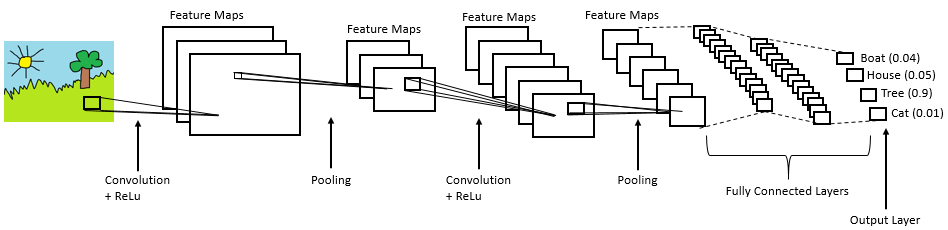
\includegraphics[width=\textwidth]{CNN.png}\caption{Base CNN}\label{fig:CNN}
		\end{center}
	\end{figure}

	Some of the application areas of CNN include Image Classification and Segmentation, Object Detection, Video Processing, Natural Language Processing, and Speech Recognition.
	
	Inception v1 to proposed by a group of researchers of Google, University of Michigan, University of North Carolina when joined in the ILSVRC 2014 competition. 
	
	GoogleNet regulates the computations by adding a bottleneck layer of 1x1 convolutional filter, before employing large size kernels.
	
	Inception Layer is a combination of all those layers (namely, 1×1 Convolutional layer, 3×3 Convolutional layer, 5×5 Convolutional layer) with their output filter banks concatenated into a single output vector forming the input of the next stage.
	
	Inception v1 included 27 layers deep with 5M parameters. \cite{ref1} 
	\newpage
	\section{Inception v1 architecture.}
		% them anh vao day
	\begin{figure}[h]
		\begin{center}
			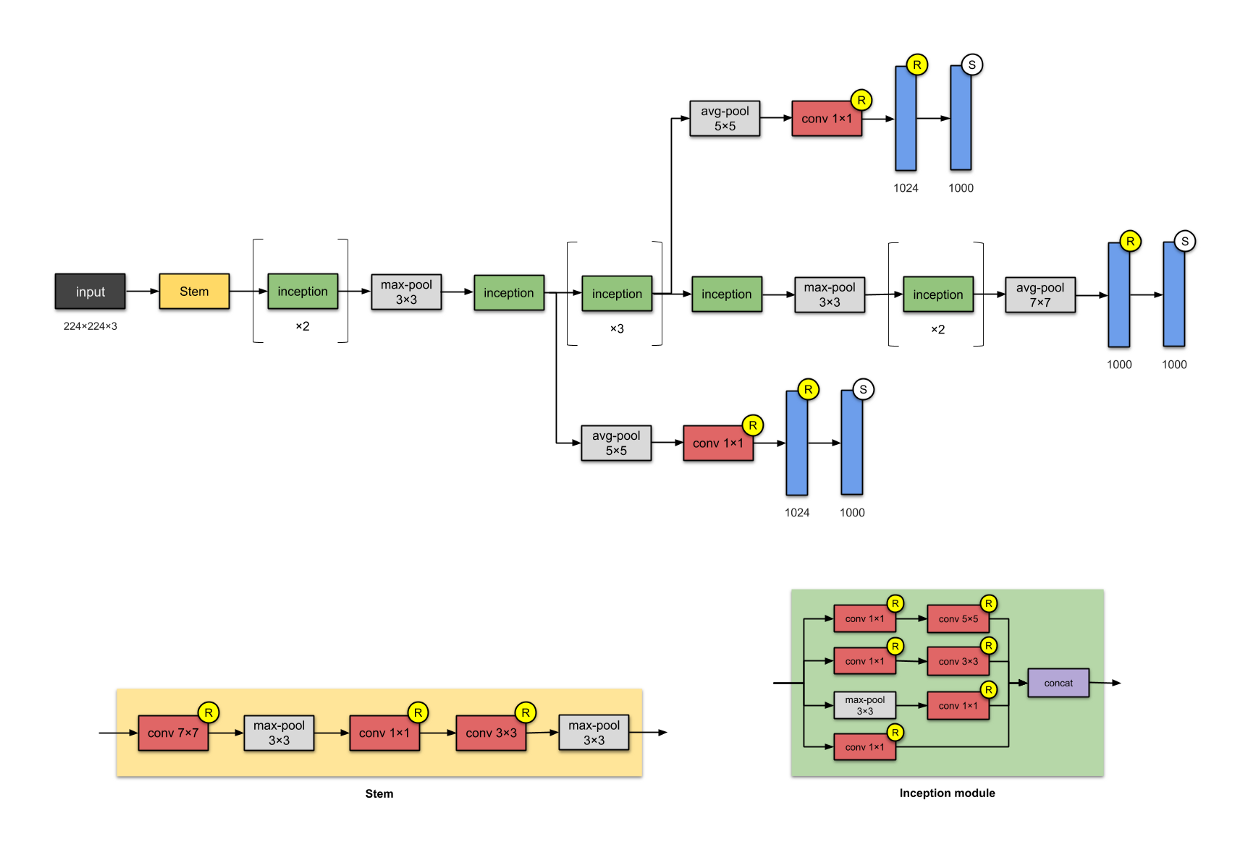
\includegraphics[width=\textwidth,height=8cm]{A.png}\caption{This figure is based on architecture in paper \cite{ref1}}\label{fig:A}
		\end{center}
	\end{figure}

	\begin{figure}[h]
		\begin{center}
			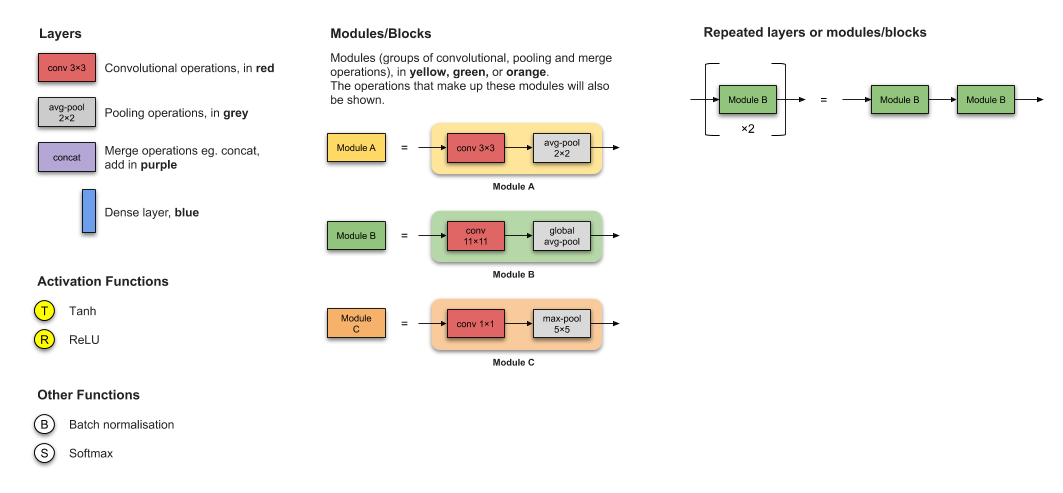
\includegraphics[width=\textwidth,height=8cm]{B.png}\caption{Description}\label{fig:B}
		\end{center}
	\end{figure}
	\newpage
	\begin{figure}[h]
		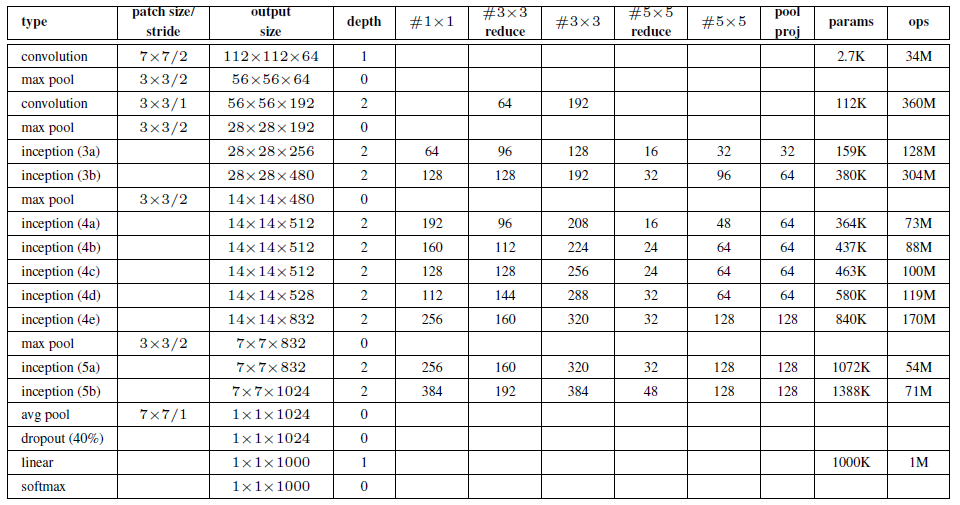
\includegraphics[width=\textwidth]{C.png}\caption{Configuration}\label{fig:C}
	\end{figure}
	\begin{figure}[h]
	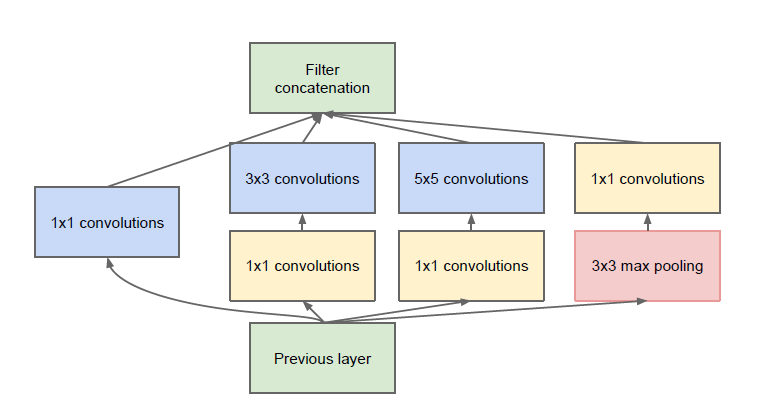
\includegraphics[width=\textwidth,height=8cm]{inception.png}\caption{Reduce computation costs by introducing a 1 x 1 convolution}\label{fig:inception}
	\end{figure}			

	\section{Layers}.
	\subsection{Convolution layers}
	In a CNN, the input is a tensor with a shape: (number of inputs) x (input height) x (input width) x (input channels). After passing through a convolution layer, the image becomes abstracted to a feature map, also called an activation map, with shape: (number of inputs) x (feature map height) x (feature map width) x (feature map channels). Example: No padding and stride is 1.
	
	\begin{figure}[ht]
		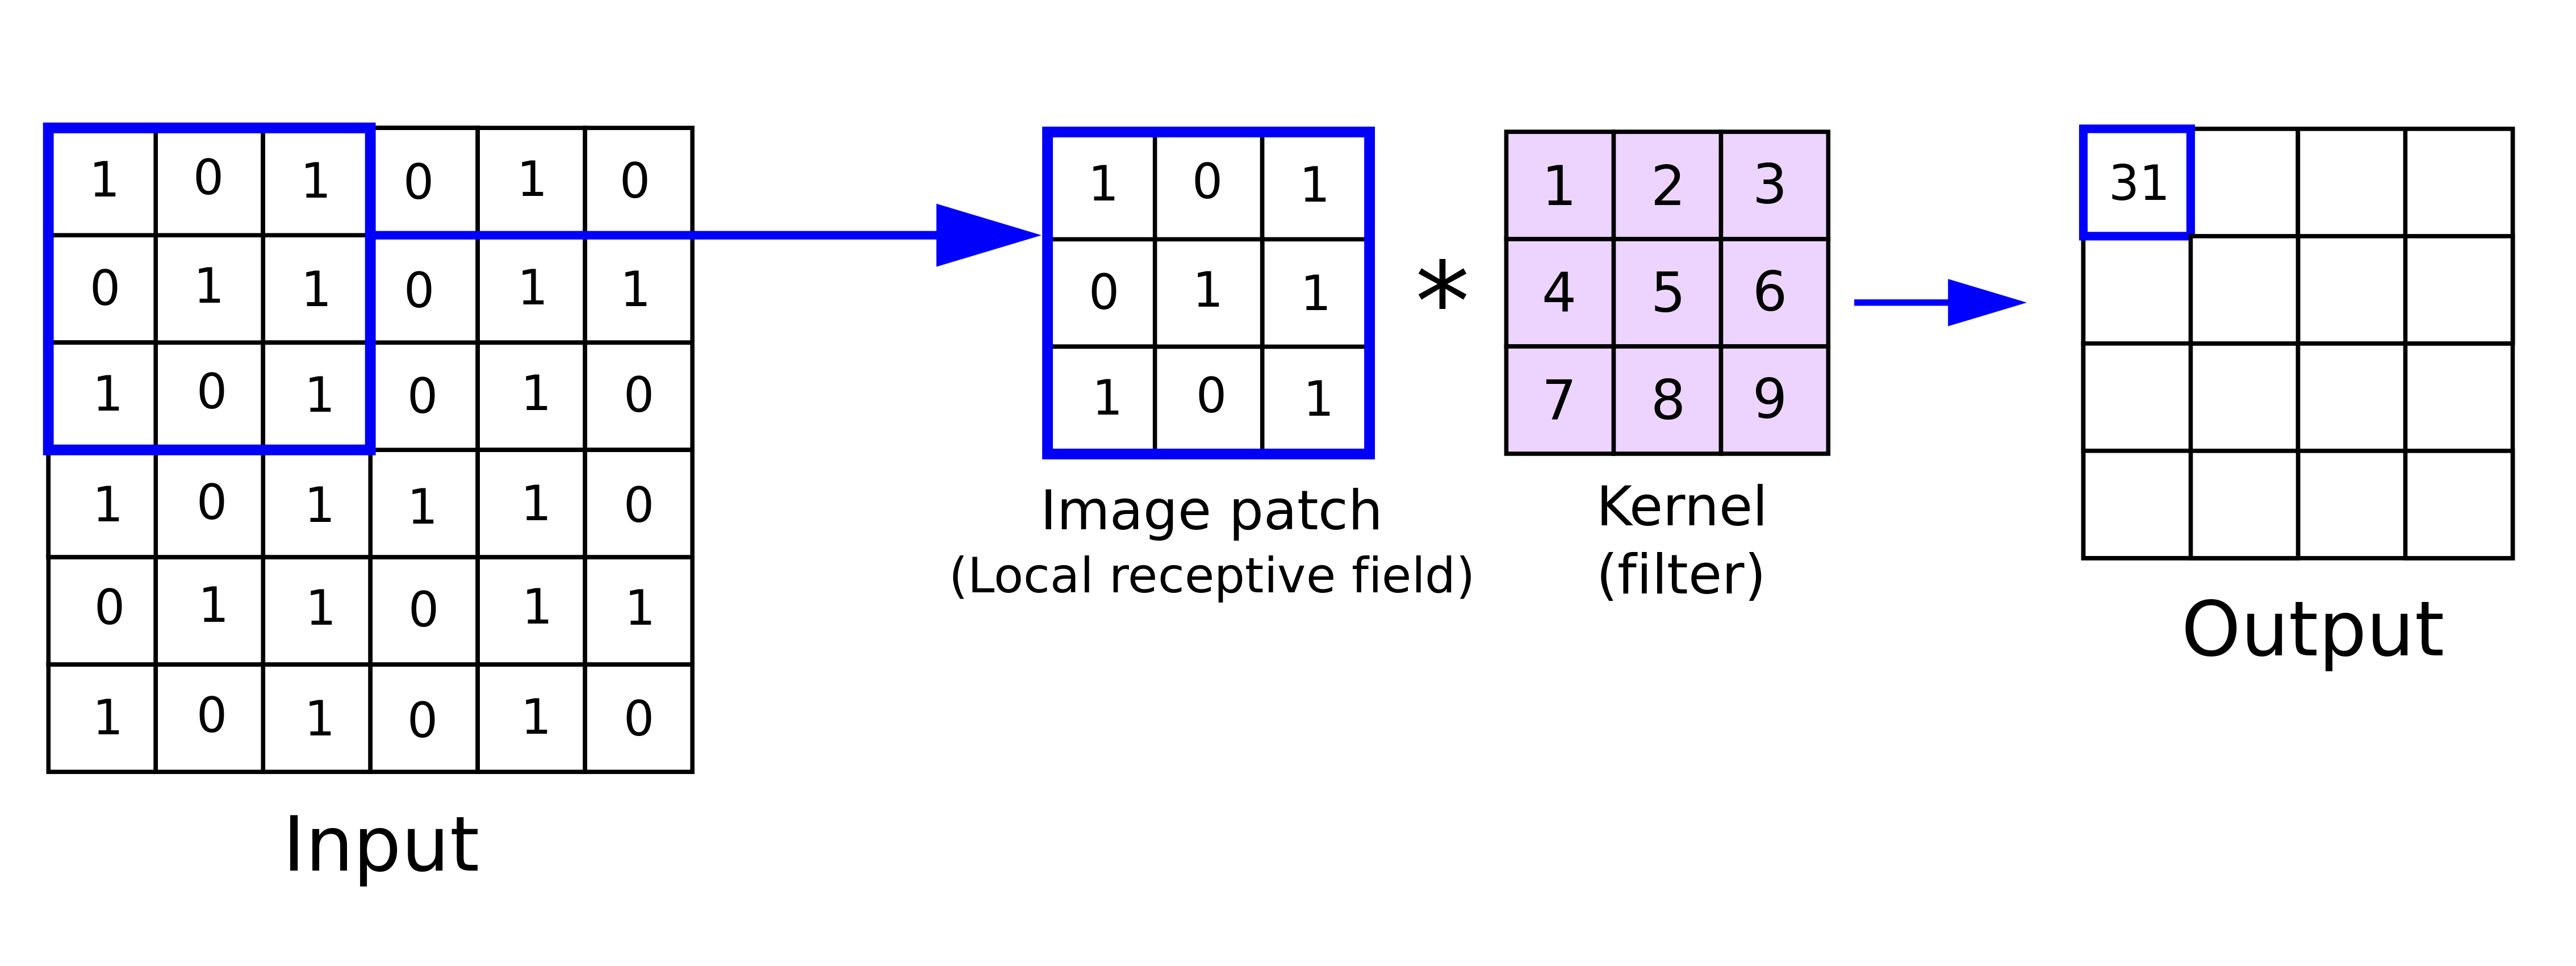
\includegraphics[width=\textwidth]{conv.png}\caption{Convolution layer}\label{fig:conv}
	\end{figure}
	\subsection{Pooling layers}
	Pooling or down-sampling is an interesting local operation. It sums up similar information in the neighborhood of the receptive field and outputs the dominant response within this local region. There are two common types of pooling in popular use: max and average. Max pooling often to use preserving the importantly features. Average pooling often to use reducing the values. 
	Example: pooling layer 2x2, stride = 2.
	\begin{figure}[h]
		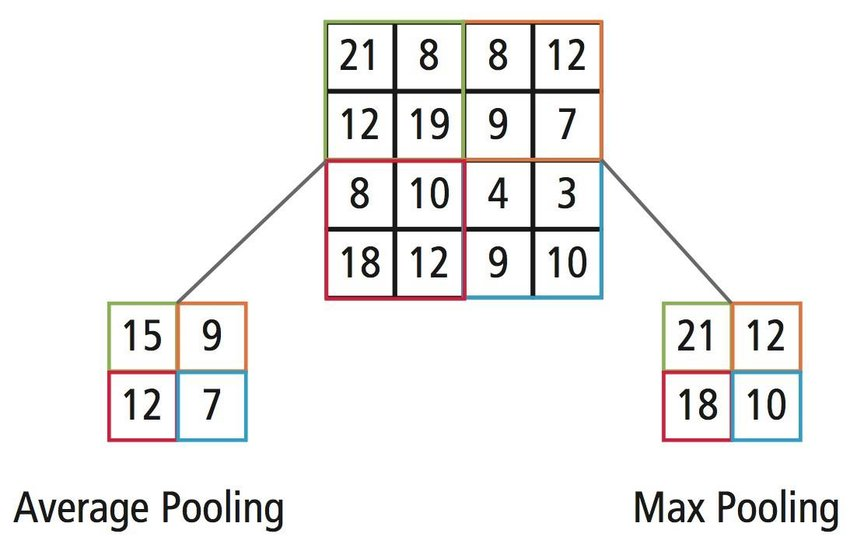
\includegraphics[width=\textwidth,height=7cm]{pooling.png}\caption{Pooling layer}\label{fig:pooling}
	\end{figure}
	
	\subsection{Activation Function}
	Activation function serves as a decision function and helps in learning of intricate patterns. The
	selection of an appropriate activation function can accelerate the learning process. There are many functions like ReLU, Sigmoid, Tanh, Leaky ReLU, Maxout. ReLU is often preferred to other functions because it trains the neural network several times faster without a significant penalty to generalization accuracy.
	\begin{figure}[h]
		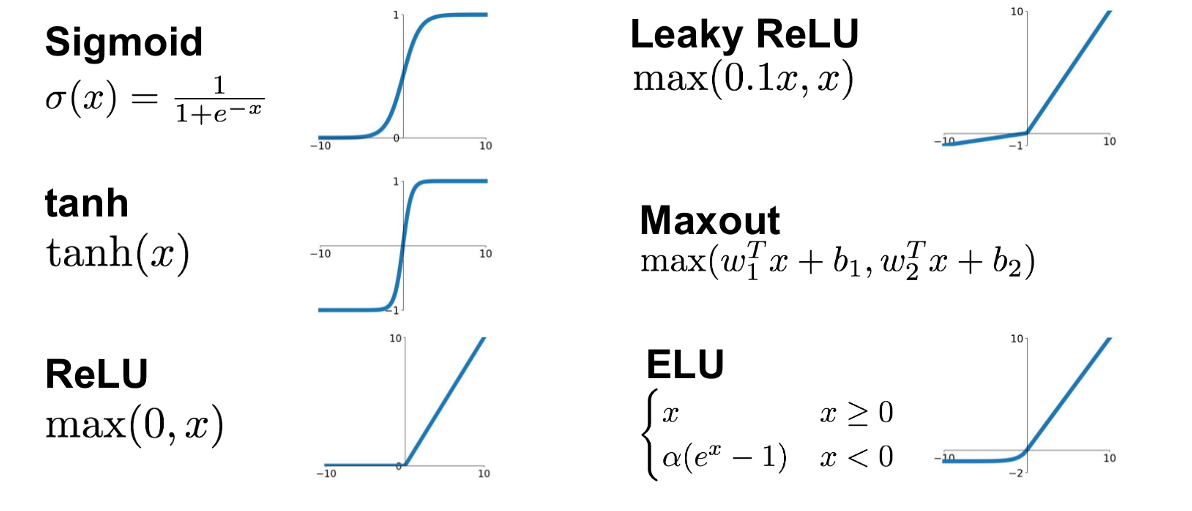
\includegraphics[width=\columnwidth]{activation-functions.png}\caption{Activation function}\label{fig=active}
	\end{figure}
	\subsection{Fully Connected layers}
	Fully connected layers connect every neuron in one layer to every neuron in another layer. The flattened matrix goes through a fully connected layer to classify the images.
	\begin{figure}[h]
		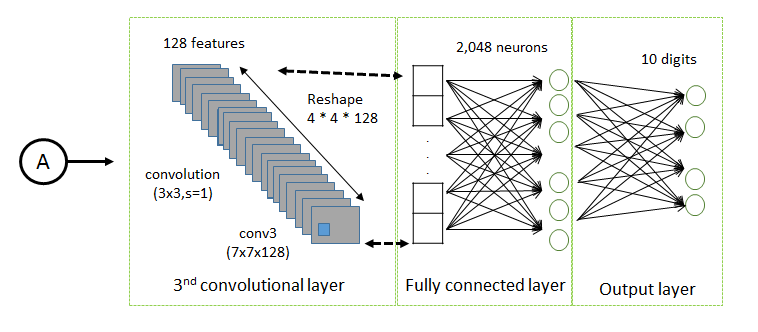
\includegraphics[width=\textwidth]{full.png}\caption{Fully Connected layer}\label{fig:full}
	\end{figure}
	
	\chapter{Ojectives}
	\begin{itemize}
		\item Understand CNN and Inception v1 architecture theory.
		\item Can use python, mathlab... to simulation, do the architecture.
		\item Using the verilog code to build Inception v1 to classification input picture 224x224x3 (RGB), output in 10 classes, datasets: CIFAR-10.
	\end{itemize}
	
	
	\chapter{Implement and Result}
%	\chapter{Results}
%	
%	\section{Achievement}
	
%	\begin{table}[h]
%		\renewcommand{\arraystretch}{1.3}
%		\caption{Example of format}
%		\label{tb::invocation}
%		\begin{center}
%			\begin{tabular}{|c|C{1cm}|C{2cm}|C{1cm}|C{1cm}|C{1cm}|}
%				\hline
%				\multirow{2}{2cm}{No. of processor}&\multirow{2}{1cm}{Up (\%)}&\multirow{2}{2cm}{No. of instance}&\multicolumn{3}{c|}{No. of scheduler invocation}\\
%				\cline{4-6}
%				& & &{\bf LAA}&{\bf Pfair}&{\bf RUN}\\
%				\hline
%				\multirow{5}{1cm}{4}&{60}&{4117}&\multirow{5}{1cm}{1000}&\multirow{5}{1cm}{10000}&{3955}\\
%				\cline{2-3}\cline{6-6}
%				{}&{70}&{4701}&{}&{}&{3726}\\
%				\cline{2-3}\cline{6-6}
%				{}&{80}&{4402}&{}&{}&{3806}\\
%				\cline{2-3}\cline{6-6}
%				{}&{90}&{2269}&{}&{}&{2077}\\
%				\cline{2-3}\cline{6-6}
%				{}&{100}&{3969}&{}&{}&{3743}\\
%				\hline
%				\multirow{5}{1cm}{32}&{60}&{19209}&\multirow{5}{1cm}{1000}&\multirow{5}{1cm}{10000}&{7953}\\
%				\cline{2-3}\cline{6-6}
%				{}&{70}&{22909}&{}&{}&{8368}\\
%				\cline{2-3}\cline{6-6}
%				{}&{80}&{29111}&{}&{}&{8657}\\
%				\cline{2-3}\cline{6-6}
%				{}&{90}&{34359}&{}&{}&{8998}\\
%				\cline{2-3}\cline{6-6}
%				{}&{100}&{33931}&{}&{}&{8868}\\
%				\hline
%			\end{tabular}
%		\end{center}
%	\end{table}
	
	
%	\section{Difficulties}
%
%	
%	\section{Discussion}

	
	\newpage
	
	%\input {References}
	\begin{thebibliography}{10}
		\bibitem{ref1}
		Christian Szegedy, Wei Liu, Yangqing Jia, Pierre Sermanet, Scott Reed, Dragomir Anguelov, Dumitru Erhan, Vincent Vanhoucke, Andrew Rabinovich. Google, University of Michigan, University of North Carolina. \enquote{Going Deeper with Convolutions,} 2015 IEEE Conference on Computer Vision and Pattern Recognition (CVPR).
		\bibitem{ref2}
		Asifullah Khan, Anabia Sohail, Umme Zahoora1 and Aqsa Saeed Qureshi, \enquote{A Survey of the Recent Architectures of Deep Convolutional Neural Networks,} Artificial Intelligence Review.
	\end{thebibliography}
\end{document}